\documentclass[article]{memoir}
\renewcommand{\cftchapterdotsep}{\cftdotsep}% Chapters should use dots in ToC
%\let\subsubsection\subsection
%\let\subsection\section % undo article option change of divisions
%\let\section\chapter    % ditto
\usepackage{xcolor}
\usepackage[utf8]{inputenc}
\usepackage{array}
\usepackage{ragged2e}
\usepackage[portuguese]{babel}
\usepackage{emoji}
\usepackage[nolist]{acronym}
\usepackage{float}
\usepackage{caption}
\footnotesinmargin % set footnotes in the margin
\usepackage{graphicx}
\usepackage{makeidx}
\usepackage{tcolorbox}
\usepackage{enumitem}
\setlist[enumerate]{label*=\arabic*.}
\usepackage{fancyhdr}
\usepackage{tikz}
\usetikzlibrary{shapes.geometric, arrows}
\usepackage{subcaption}
\usepackage{caption}
\newcounter{run}
\InputIfFileExists{\jobname.runs}{}{}
\stepcounter{run}

\usepackage{atveryend}
\usepackage{newfile}
\AtVeryEndDocument{%
	\newoutputstream{runs}%
	\openoutputfile{\jobname.runs}{runs}%
	\addtostream{runs}{\string\setcounter{run}{\number\value{run}}}%
	\closeoutputstream{runs}%
}



\pagestyle{fancy}
\fancyhf{} % clear all fields
\fancyhead[L]{\rightmark}
\fancyhead[R]{\thepage}

\renewcommand{\subsectionmark}[1]{%
	\markright{\MakeUppercase{\thesubsection.\ #1}}}%




\newcommand*\lowercasecapitals[1]{\MakeLowercase{\large\scshape#1}}
\setsecheadstyle{\lowercasecapitals}


\usepackage[hyperpageref]{backref}
\usepackage{listings}
\renewcommand{\lstlistingname}{Código}
\usepackage{xcolor}
\usepackage{ifpdf}
%\ifpdf
%\pdfinfo{
	%	/Author (Cledson de Sousa)
	%	/Title  (Apostila de Geência de Redes e Engenharia de Tráfego)
	%	/CreationDate (D:20240407)
	%	/Subject (Gerência de Redes e Engenharia de Tráfego)
	%	/Keywords (Tráfego e redes)
	%}
%\fi
\usepackage{multicol}
\usepackage{hyperref}
\hypersetup{
	pdftitle={Visualização e Representação de Dados},
	pdfsubject={Representação de dados},
	pdfauthor={Prof.: Cledson de Sousa},
	pdfkeywords={análise de dados, gráficos}
	%pdfdate = {april 07, 2024}
}

\setcounter{secnumdepth}{3}

% Definição das cores no estilo GitHub
\definecolor{backcolour}{rgb}{0.95, 0.95, 0.92}
\definecolor{codegreen}{rgb}{0,0.6,0}
\definecolor{codeblue}{rgb}{0.24, 0.37, 0.78}
\definecolor{codegray}{rgb}{0.5, 0.5, 0.5}
\definecolor{codepurple}{rgb}{0.58, 0, 0.82}
\definecolor{magenta}{rgb}{1.0, 0.0, 1.0}



\makeindex % Inicializa o sistema de índice remissivo



\begin{document}
	
% Estilo de listagem no estilo GitHub
\lstdefinestyle{github}{
	backgroundcolor=\color{backcolour},   
	commentstyle=\color{magenta},       % Define a cor dos comentários como verde
	keywordstyle=\color{codeblue},
	numberstyle=\tiny\color{codegray},
	stringstyle=\color{codepurple},
	basicstyle=\ttfamily\footnotesize,
	breakatwhitespace=false,         
	breaklines=true,                 
	captionpos=b,                    
	keepspaces=true,                 
	numbers=left,                    
	numbersep=5pt,                  
	showspaces=false,                
	showstringspaces=false,
	showtabs=false,                  
	tabsize=2,
	morecomment=[l]{\%}
	morecomment=[l]{;}
	              % Define o símbolo de comentário como "%"
}
\lstset{style=github}

%\cite{abntex2classe}
% Capa

	\begin{titlingpage} % Ambiente para a capa
		\centering
		\vspace*{1cm}
		\Huge Universidade Federal Fluminense \\
		%\Large Apostila de Gerência de Redes e Engenharia de Tráfego
		\vspace{2cm}
		% Espaço reservado para figura/logo
		\vspace{1cm} % Ajuste este espaço conforme necessário
		
\includegraphics[width=0.8\textwidth]{figs/uffdataacademy.png}
		% Descomente a linha acima e substitua "caminho-para-sua-figura-aqui.png" pelo caminho correto do arquivo de imagem que você deseja incluir
		
		\vspace{1cm}
		\Huge \textbf{Gerência de Redes e Engenharia de Tráfego}\\[0.5cm] % Título

		
		\vfill
		\Large Professor Cledson de Sousa\\[0.5cm] % Seu nome
		Versão: 0.1.\therun -- 13 de maio/2024 -- Até MPLS.
		%Data do Curso: \today % Ou coloque a data específica
		

		
	\end{titlingpage}	
\setcounter{secnumdepth}{4}
\setcounter{tocdepth}{4}
	\tableofcontents*



%\section*{Lista de Acrônimos}

\begin{acronym}
%\begin{multicols}{2}
	\begin{footnotesize}
	\acro{AAL}[AAL]{\textit{Adaptation Layer}} 
	\acro{ATM}[ATM]{\textit{Asynchronous Transfer Mode}}
	\acro{BGP}[BGP]{\textit{Border Gateway Protocol}}
	\acro{DevOps}[DevOps]{\textit{Development and Operations}}
	\acro{ET}[ET]{Engenharia de Tráfego}
	\acro{FCAPS}[FCAPS]{\textit{Fault, Configuration, Accounting, Performance, and Security}}
	\acro{IGP}[IGP]{\textit{Interior Gateway Protocol}}
	\acro{IP}[IP]{\textit{Internet Protocol}}
	\acro{IETF}[IETF]{\textit{Internet Engineering Task Force}}
	\acro{MPLS}[MPLS]{\textit{Multiprotocol Label Switching}}
	\acro{NFV}[NFV]{\textit{Network Functions Virtualization}}
	\acro{RFC}[RFC]{\textit{Request for Comments}}
	\acro{TE}[TE]{Traffic Engineering}
	\acro{QoS}[QoS]{\textit{Quality of Service}}
	\acro{SDN}[SDN]{\textit{Software-Defined Networking}}
	\acro{SLA}[SLA]{\textit{Service Level Agreement}}
	\acro{VLAN}[VLAN]{\textit{Virtual Local Area Network}}
	\acro{VPN}[VPN]{\textit{Virtual Private Network}}
\end{footnotesize}
%\end{multicols}
\end{acronym}

\section*{Prefácio}

Caros futuros engenheiros, 

Bem-vindos ao curso de Gerência de Redes e Engenharia de Tráfego, uma disciplina  criada para introduzir os conceitos fundamentais e práticas avançadas da controle de tráfego. administração e gerência de modernas infraestruturas de rede. Este curso, estruturado com uma mistura equilibrada de aulas em classe e extra-classe, cobre uma carga horária total de 60 horas, das quais 40 horas são dedicadas a conceitos teóricos e 20 horas a aplicações fora de sala. Então o objetivo é proporcionar aos alunos uma compreensão abrangente dos modelos de gerência de redes, monitoramento, auditoria e a engenharia de tráfego necessária para lidar com o encaminhamento do tráfego.


Esta apostila, embora tenha um caráter acadêmico, não possui a pretensão de ser extremamente rigorosa, especialmente na forma. O autor empenhou-se em dar o devido crédito a todas as fontes utilizadas; no entanto,por vezes, estende-se o texto sem as devidas citações específicas dos autores originais. Então peço que aceitem as escusas do autor, pois muitas das fontes são os textos originais presentes nos locais onde as figuras foram extraídas. Além disso, diversas explicações são fruto do esforço do autor em dissecar os diagramas, que frequentemente simplificam o verdadeiro encaminhamento dos pacotes.

Ao longo do texto há diversos sinais de parada \emoji{stop-sign}, em notas de margem, gráficos, figuras e outros sinais. Estes sinais lá estão  para o leitor desopilar, se você chegou em um desses sinais parabéns! É por que você já leu o suficiente, nesse momento é bom parar, descontrair, visitar os sites e sair um pouco do texto, naturalmente deve-se retornar ao texto tão logo possível. Essa estratégia funciona comigo!
Um curso leve, produtivo, enriquecedor e sem reprovações. É o que desejo!

\textbf{Sobre o autor:}

O autor recebeu seu título de Doutor em Computação pela Universidade Federal Fluminense (UFF) em 2019, e seus títulos de graduação e mestrado em Engenharia de Telecomunicações pela mesma universidade, em 1997 e 2013. Com mais de 30 anos de experiência na indústria de telecomunicações, desde 2021 é Professor Adjunto do Departamento de Engenharia de Telecomunicações da Universidade Federal Fluminense. Seus interesses de pesquisa atuais incluem redes de sensores sem fio, SDN, rádios cognitivos e CSI.\mbox{}\\

\textbf{Plataformas:}

\begin{itemize}
	\item LinkedIn: \url{https://www.linkedin.com/in/cledsonsousa}
	\item Página pessoal: \url{https://cledsonsousa.github.io}
	\item Currículo Lattes: \url{http://lattes.cnpq.br/7195080748145566}
\end{itemize}

\newpage
\chapter{Introdução}
\section{O Conceito de Camadas}
O conceito de camadas (\textit{layering}) é fundamental para a visualização de dados, Vamos explorar como esse conceito facilita essas representações:

\paragraph*{Separação de Elementos Visuais:}\mbox{}\\
Camadas permitem separar diferentes elementos visuais em uma visualização de dados. Por exemplo, ao representar um conjunto de dados, uma camada pode ser usada para mostrar os valores médios, enquanto outra camada pode ser usada para mostrar a variação desses valores (como barras de erro ou intervalos de confiança). Isso ajuda a distinguir claramente entre os dados principais e as informações auxiliares que podem por exemplo  representar incerteza.

\paragraph*{Flexibilidade na Visualização:}\mbox{}\\
O uso de camadas oferece flexibilidade na criação de gráficos complexos. Diferentes tipos de representações visuais, como pontos de dados, linhas de tendência, e intervalos de confiança, podem ser adicionados ou removidos conforme necessário. Isso permite que os visualizadores ajustem a complexidade da visualização com base em suas necessidades específicas.

\begin{figure}[ht]
	\centering
	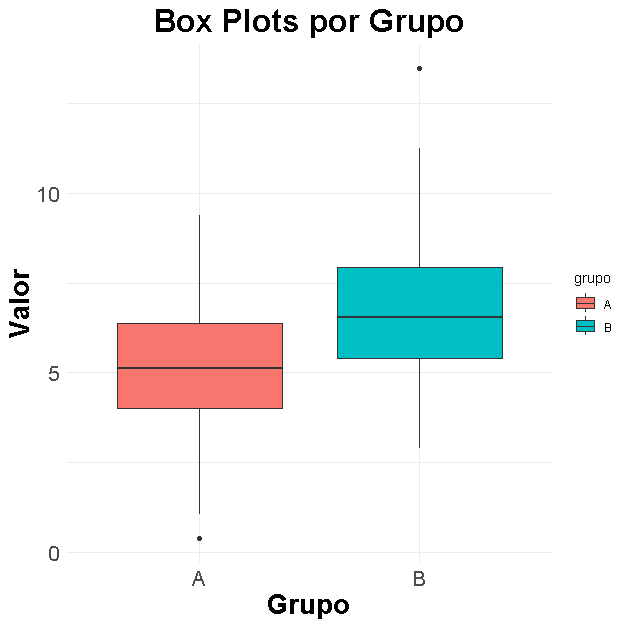
\includegraphics[width=0.5\linewidth]{figs/layers_box_plt_example}
	\caption{}
	\label{fig:layersboxpltexample}
\end{figure}


\paragraph*{Exemplo Prático:}\mbox{}\\
 \textit{Box plots} como o apresentados na Figura 	\ref{fig:layersboxpltexample}, por exemplo, utilizam camadas. A camada do \textit{box plot} mostra a mediana e os quartis, enquanto camadas adicionais indicam \textit{outliers}.


	
\section{Variação e Incertezas}


O conceito de camadas também facilita a representação da variação estatística e da incerteza. É importante se lembrar que dados experimentais tipicamente apresentam alguma incerteza  e a visualização e representação destes dados deve "caracterizar a magnitude dessa incerteza em relação aos dados reais  \cite{wainer1996depicting}. 

Os autores infelizmente mostram resultados que em muitos trabalhos as figuras publicadas não atendem a esse padrão, especialmente à medida que a dimensionalidade dos dados aumenta \cite{allen2012data}. Quando o objetivo de uma visualização é comparar uma quantidade medida ou derivada entre categorias ou condições, deve-se incluir um elemento (são as \textit{geom} do \texttt{ggplot}) gráfico retratando a quantidade e um segunda elemento  retratando a incerteza da quantidade. Note que, sem a representação da incerteza, uma comparação visual precisa não é possível, os leitores podem tirar conclusões incorretas ou mal informadas.

A variação e a incerteza podem ser retratadas com uma variedade de \textit{geoms}, mas são mais comumente exibidas com barras de erro. Infelizmente, não há um padrão único para o que a barra de erro deve representar já que há uma pluralidade esmagadora de significados possíveis, como desvio padrão (DP) da amostra, erro padrão da média (EPM) ou simplesmente erro padrão, Intervalo de Confiança (IC) paramétrico de $100(1 − \alpha)\%$ , intervalo de probabilidade bayesiano, um intervalo de previsão, etc. Cada quantidade tem sua própria interpretação estatística

Portanto, ao usar barras de erro, certifique-se de que (1) a quantidade codificada pela barra é consistente com o objetivo da visualização e (2) a quantidade é definida de forma inequívoca. Em relação ao primeiro ponto, oferecemos as seguintes diretrizes ao usar barras de erro para retratar a variação de uma estimativa de parâmetro ou a variação dos dados.
\begin{figure}[ht]
	\centering
	\begin{minipage}{0.7\textwidth} % Ajuste a largura total da figura aqui
		\begin{subfigure}[b]{0.45\textwidth}
			\centering
			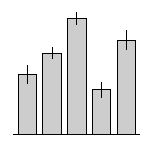
\includegraphics[width=\textwidth]{figs/error_bar_example}
			\caption{Gráficos de barra com barra de erros.}
			\label{fig:sub1}
		\end{subfigure}
		\hfill
		\begin{subfigure}[b]{0.45\textwidth}
			\centering
			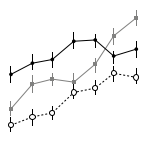
\includegraphics[width=\textwidth]{figs/error_line_example}
			\caption{Gráficos de linhas com barra de erros.}
			\label{fig:sub2}
		\end{subfigure}
	\end{minipage}
	\caption{as barras normalmente para comparar categorias e as linhas para comparar grupos e tendências.}
	\label{fig:ex_bar_lines}
\end{figure}
\subsection{Intervalo de Confiança e Nível de Significância}
Se o interesse for estimar um parâmetro populacional, como a média ou a variância, então a variação da estimativa (isto é, a distribuição amostral da estatística) é desejada. Exemplos de barras de erro adequadas incluem o EPM ou um IC paramétrico ou \textit{bootstrap} de 95\%, como visto em visualizações que enfatizam comparações (Figura	\ref{fig:ex_bar_lines}). ICs paramétricos devem ser usados apenas se os dados atenderem às suposições do modelo subjacente, caso contrário, um \textit{bootstrap} (ou outra estratégia para aproximar a distribuição amostral) deve ser usado\footnote{E o que é $\alpha$? o nível de significância: 
	$\alpha$ é a probabilidade de cometer um erro tipo I, que ocorre quando rejeitamos a hipótese nula ($H_0$)
	 quando ela é verdadeira. \textbf{Em outras palavras, é a taxa de falso positivo permitida.}}. 

\begin{tcolorbox}
	\textbf{IC um conceito muitas vezes mal entendido \cite{belia2005} e \cite{hoekstra2014}}
	
	Um intervalo de confiança de $100(1 − \alpha)\%$  para um parâmetro populacional é um intervalo calculado a partir dos dados amostrais que, em $100(1 − \alpha)\%$ das amostras possíveis, conteria o verdadeiro valor do parâmetro.
	
	\textbf{Isto é:} Suponha que você calcule a média de alturas de uma amostra de 100 pessoas e obtenha uma média de 170 cm com um desvio padrão de 10 cm. Um intervalo de confiança de 95\% pode ser calculado, e você pode obter algo como (168 cm, 172 cm). Isso significa que, se você repetisse esse experimento várias vezes, 95\% dos intervalos de confiança calculados conteriam a verdadeira média populacional (nesse caso 170 cm).
	
\end{tcolorbox} 

Um outro exemplo de interpretação geométrica dos intervalos de confiança são a sua sobreposição ou não entre duas amostras.

\begin{tcolorbox}
	\textbf{A sobreposição dos ICs  \cite{cumming2007} e \cite{krzywinski2013}}
	
	Um intervalo de confiança de $100(1 − \alpha)\%$  para um parâmetro populacional é um intervalo calculado a partir dos dados amostrais que, em $100(1 − \alpha)\%$ das amostras possíveis, conteria o verdadeiro valor do parâmetro.
	
	\textbf{Isto é:} Suponha que você calcule a média de alturas de uma amostra de 100 pessoas e obtenha uma média de 170 cm com um desvio padrão de 10 cm. Um intervalo de confiança de 95\% pode ser calculado, e você pode obter algo como (168 cm, 172 cm). Isso significa que, se você repetisse esse experimento várias vezes, 95\% dos intervalos de confiança calculados conteriam a verdadeira média populacional (nesse caso 170 cm).
	
\end{tcolorbox} 



 Enquanto ICs de 95\% não sobrepostos indicam uma diferença significativa (sob um modelo de probabilidade normal), o inverso não é verdadeiro — dependendo do tamanho da amostra, as barras de IC podem se sobrepor em até 50\% e ainda atender aos critérios de significância \cite{cumming2007}.



\begin{figure}[ht]
	\centering
	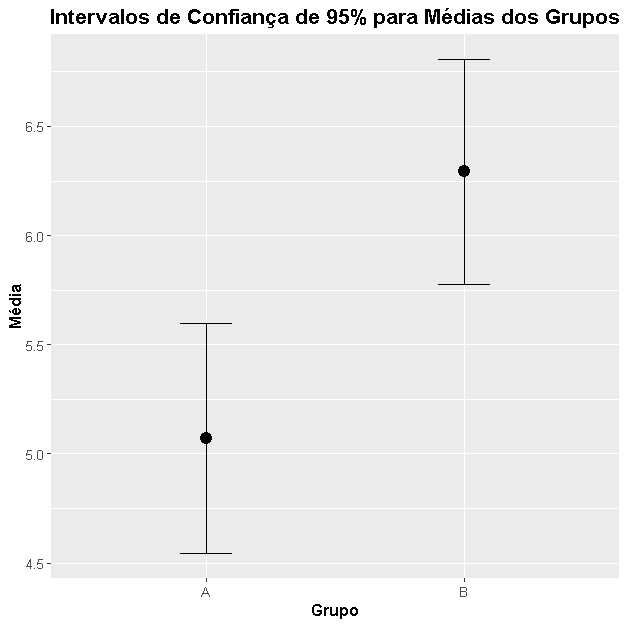
\includegraphics[width=0.7\linewidth]{figs/IC_sobrep_visual}
	\caption{ICs de 95\% não sobrepostos indicam uma diferença significativa (sob um modelo de probabilidade normal).}
	\label{fig:icsobrepvisual}
\end{figure}

As barras de erro são destinadas a indicar a faixa de valores prováveis para alguma estimativa ou medição. Elas se estendem horizontalmente e/ou verticalmente a partir de um ponto de referência que representa a estimativa ou medição. No entanto o  erro ou o IC podem ser mostrado de várias maneiras, como por pontos barras ou faixas. Barras de erro graduadas mostram múltiplas faixas ao mesmo tempo, onde cada faixa corresponde a um grau diferente de confiança. Elas são, na prática, múltiplas barras de erro com diferentes espessuras de linha plotadas umas sobre as outras \cite{Wilke2019}.

\begin{figure}[ht]
	\centering
	\includegraphics[width=1\linewidth]{"../../vis_rep_data/apostila/figs/band _and_violin1"}
	\caption{três diferentes visualizações que utilizam intervalos de confiança para representar a incerteza e variabilidade dos dados.}
	\label{fig:band-andviolin1}
\end{figure}
Os gráficos apresentados na Figura \ref{fig:band-andviolin1}  são três diferentes visualizações que utilizam intervalos de confiança para representar a incerteza e variabilidade dos dados.
a Figura \ref{fig:band-andviolin1}a) mostra um Gráfico de Dispersão com Banda de Confiança: As bandas de confiança servem para mostrar a incerteza na relação entre duas variáveis. Já a Figura \ref{fig:band-andviolin1}b) do Gráfico de Meio-Violino mostra a metade da distribuição dos dados para diferentes categorias, destacando a densidade dos dados e os intervalos interquartis.
 E o da Figura \ref{fig:band-andviolin1}c), o Gráfico de Violino Completo, apresenta uma visão completa da distribuição dos dados, facilitando uma comparação detalhada entre as categorias.

Esses gráficos são úteis para entender não apenas os valores médios, mas também a variabilidade, a distribuição e a incerteza dos dados, proporcionando uma compreensão mais completa e detalhada das características dos dados analisados.
\chapter{Introdução a Análise de Dados}

Experimentos na nossa área (Engenharia) tipicamente nos inundam com dados muitas vezes difíceis de entender e quiçá explicar. O objetivo aqui é escrutinar o método, a lógica, a arte e a prática da análise e representação de dados, fornecendo as habilidades e ferramentas essenciais para examinar dados e resolver problemas. Concordamos com a filosofia de "aprender fazendo" para uma melhor compreensão da análise de dados\footnote{Este capítulo foi fortemente baseado em \cite{brown2021statistics} de David Brown \emoji{backhand-index-pointing-down} (ver Figura \ref{fig:mrbrown}).}.


\begin{marginfigure}
	\centering
	
\includegraphics[width=0.7\linewidth]{../../vis_rep_data/apostila/figs/mr_brown}
	\caption{Mr. Brown  Tem mais de 20 anos de experiência como avaliador estatístico na MHRA e, antes do Brexit, foi membro do grupo de trabalho de bioestatística e do grupo de trabalho de aconselhamento científico da EMA. Ele fez parte do grupo que formulou a orientação recentemente publicada da MHRA sobre dados do mundo real.}
	\label{fig:mrbrown}
\end{marginfigure}

\section{Casos Reais}
Ao perceber um aumento na quantidade de propagandas de fraldas, fórmulas infantis e macacões da Target, o destinatário liga para a Target perguntando por que estão enviando tanta publicidade voltada para bebês (já fazia anos que não havia um bebê em casa). A Target explicou que os dados recentes de compras indicavam que havia uma mulher grávida na residência. Uma semana após ligar para a Target, ele descobre que sua filha está grávida.

Em um cenário como os dos surtos de H1N1, Ebola, Zika ou COVID-19, o peíodo comum de 2 semanas de análise é longo demais. Uma equipe do Google permitiu que a Internet descobrisse onde os surtos ocorriam. Para desenvolver seu modelo, eles rastrearam a disseminação do H1N1 e correlacionaram com termos de busca na Internet: febre alta, tosse e dores. Informando as autoridades quando e onde exatamente o novo surto de gripe estava ocorrendo.

Para ajudar a reduzir o crime em Chicago. Equipados com sensores que localizam disparos de armas pela cidade, junto com mapas de lojas de bebidas alcoólicas e acessos de rodovias, os analistas identificam áreas onde o crime provavelmente ocorrerá. Essa informação, combinada com dados sobre eventos esportivos televisionados, aumenta a precisão na localização de possíveis problemas\footnote{Esses e outros casos podem ser encontrados em \cite{mayer2013big}.}. 




\section{Componentes da Análise de Dados}
O foco está no processo de formação de hipóteses, teste de teorias e obtenção de inferências. Vamos abordar  essas bases de investigação por meio da visualização de dados e trabalhando em problemas reais com dados reais.

São quatro os componentes da análise de dados  nessa ordem: 
\begin{enumerate}
	\item Descrição de dados e formulação de hipóteses.
	\item Construção e estimativa de modelos. 
	\item Diagnósticos.
	\item Próxima pergunta. 
\end{enumerate}

	Existem múltiplos conceitos e técnicas (ou seja, construção e estimativa de modelos, transformação de variáveis, diagnósticos etc.). O propósito deste capítulo é introduzir as linhas gerais estratégias de uma boa análise de dados com um exemplo. 

\paragraph*{Descrição de Dados e Formulação de Hipóteses:}\mbox{}\\

Descrever dados significa, a princípio, identificar o caso típico (\textbf{tendência central}) e entender quão típico é esse caso típico (dispersão). No entanto com as novas ferramentas, deve-se ir muito além disso. Significa, entender, correlacionar e encontrar padões.
E as hipóteses? Para nós uma hipótese se referirá a uma suposição específica sobre como duas coisas estão relacionadas (por exemplo, probabilidade de acesso ao meio e vazão total). 

\paragraph*{Construção e Estimativa de Modelos:}\mbox{}\\

Modelos são versões simplificadas da realidade que nos ajudam a entender nosso mundo complexo. São argumentos  para explicar um problema empírico. Por exemplo, se queremos explicar por que alguns países têm altas taxas de homicídio, construímos um modelo que pode incluir renda, idade da população, número de policiais e eficácia do sistema judiciário. Há uma infinidade de outras possíveis causas que poderíamos incluir, mas é útil manter as coisas simples, mas em engenharia não queremos recriar a realidade; queremos apenas aproximá-la. 

\paragraph*{Diagnósticos:}\mbox{}\\
Depois de construirmos modelos e obtermos algumas estimativas, passamos para os diagnósticos. Diagnósticos são um conjunto de ferramentas que usamos para determinar se estamos usando o tipo certo de modelo. Para verificar se nosso modelo é apropriado, examinamos quão bem as previsões do nosso modelo correspondem à realidade. A diferença entre nossa previsão e a realidade é chamada de erro residual. Por exemplo, se nosso modelo faz um bom trabalho ao prever a vazão total (em bps) em todas as redes, exceto nas redes sem fio em áreas urbanas densas, os diagnósticos resultantes dirão isso. Ou seja, os resíduos para esses casos serão relativamente grandes. Talvez nossas estimativas de modelo estejam sendo excessivamente influenciadas por essas redes sem fio urbanas. Diagnósticos nos ajudam a determinar se nossas estimativas fornecem uma boa noção de como a vazão de rede realmente funciona, são o produto de alguns casos atípicos ou são o resultado de um modelo mal escolhido.

É importante lembrar que diagnósticos podem tanto detectar problemas quanto ajudar a descobrir relações interessantes, gerando explicações adicionais ou hipóteses. 

\paragraph*{As Próximas Perguntas:}\mbox{}\\
 se as estimativas que obtivemos estão corretas, então esperaríamos ver nossa variável acompanhar certo comportamento. Seguir cada conjunto de estimativas com essa declaração ajuda a descobrir explicações possíveis e hipóteses adicionais a serem testadas. Como é impossível provar qualquer coisa com total certeza, o exercício de gerar hipóteses adicionais para testar é extremamente importante. 

\section{Descrevendo e Formulando Hipóteses}
https://medium.com/number-around-us/hypothesis-testing-in-r-elevating-your-data-analysis-skills-e7256ed64178

Os testes de hipóteses constituem uma pedra angular, o teste de hipótese trata de determinar a probabilidade de que uma determinada premissa sobre um conjunto de dados seja verdadeira. É um método usado para validar ou refutar suposições, muitas vezes levando a novos \textit{insights} e entendimentos. Na sua essência, envolve a formulação de duas hipóteses concorrentes: a hipótese nula ($H_0$) e a hipótese alternativa ($H_1$).

A hipótese nula, $H_0$, representa uma crença básica. É uma afirmação de nenhum efeito ou nenhuma diferença, como “Não há diferença nas alturas médias entre duas espécies de plantas”. Em contrapartida, a hipótese alternativa, H1, representa o que procuramos estabelecer. É uma afirmação de efeito ou diferença, como ``Há uma diferença significativa nas alturas médias entre estas duas espécies".

Para decidir entre essas hipóteses, usamos um valor $p$, uma estatística crucial no teste de hipóteses. O valor p nos diz a probabilidade de observar nossos dados, ou algo mais extremo, se a hipótese nula fosse verdadeira. Um valor p (\textit{p-value}) baixo (geralmente abaixo de 0,05) sugere que os dados observados são improváveis sob a hipótese nula, levando-nos a considerar a hipótese alternativa.

No contexto do teste de correlação de Pearson, o valor $p$ desempenha um papel fundamental na determinação da significância estatística da correlação observada entre duas variáveis. O teste de Pearson avalia a força e a direção da relação linear entre duas variáveis contínuas. Ao realizar este teste, calculamos o coeficiente de correlação de Pearson (r), que pode variar de -1 a 1. No entanto, para inferir se a correlação observada é estatisticamente significativa, analisamos o valor $p$ associado.

Quando o valor p é baixo, indica que a probabilidade de obter um coeficiente de correlação tão extremo quanto o observado, se a hipótese nula de correlação zero fosse verdadeira, é pequena. Por exemplo, um valor p menor que 0,05 sugere que há menos de 5\% (0.05) de chance de a correlação observada ser devida ao acaso, fornecendo evidências contra a hipótese nula e a favor de uma correlação verdadeira entre as variáveis. Portanto, a interpretação do valor $p$ no teste de Pearson nos ajuda a decidir se podemos rejeitar a hipótese nula e aceitar a hipótese alternativa de que existe uma correlação significativa.

No entanto, o teste de hipóteses não está isento de riscos, nomeadamente erros do Tipo I e do Tipo II. Um erro Tipo I, ou falso positivo, ocorre quando rejeitamos incorretamente uma hipótese nula verdadeira. Por exemplo, concluir que um novo medicamento é eficaz quando não o é, seria um erro do Tipo I. Este tipo de erro pode levar a uma falsa confiança em tratamentos ou intervenções ineficazes.

Por outro lado, um erro Tipo II, ou falso negativo, ocorre quando não conseguimos rejeitar uma hipótese nula falsa. Isto seria como não reconhecer a eficácia de um medicamento benéfico. Os erros do tipo II podem levar à perda de oportunidades de intervenções ou tratamentos benéficos.

O valor crítico é o ponto de corte que determina a fronteira entre a região onde rejeitamos a hipótese nula ($H_0$) e a região onde não a rejeitamos, com base no nível de significância ($\alpha$) do teste. É calculado de modo que a probabilidade de cometer um erro do Tipo I (rejeitar $H_0$ quando $H_0$ é verdadeira) seja igual a $\alpha$. Por exemplo, em um teste unilateral com nível de significância de 5\% ($\alpha$ = 0.05), o valor crítico na distribuição normal padrão seria aproximadamente 1.645. Se a estatística de teste exceder este valor crítico, rejeitamos $H_0$, caso contrário, não a rejeitamos.


\begin{figure}[ht]
	\centering
	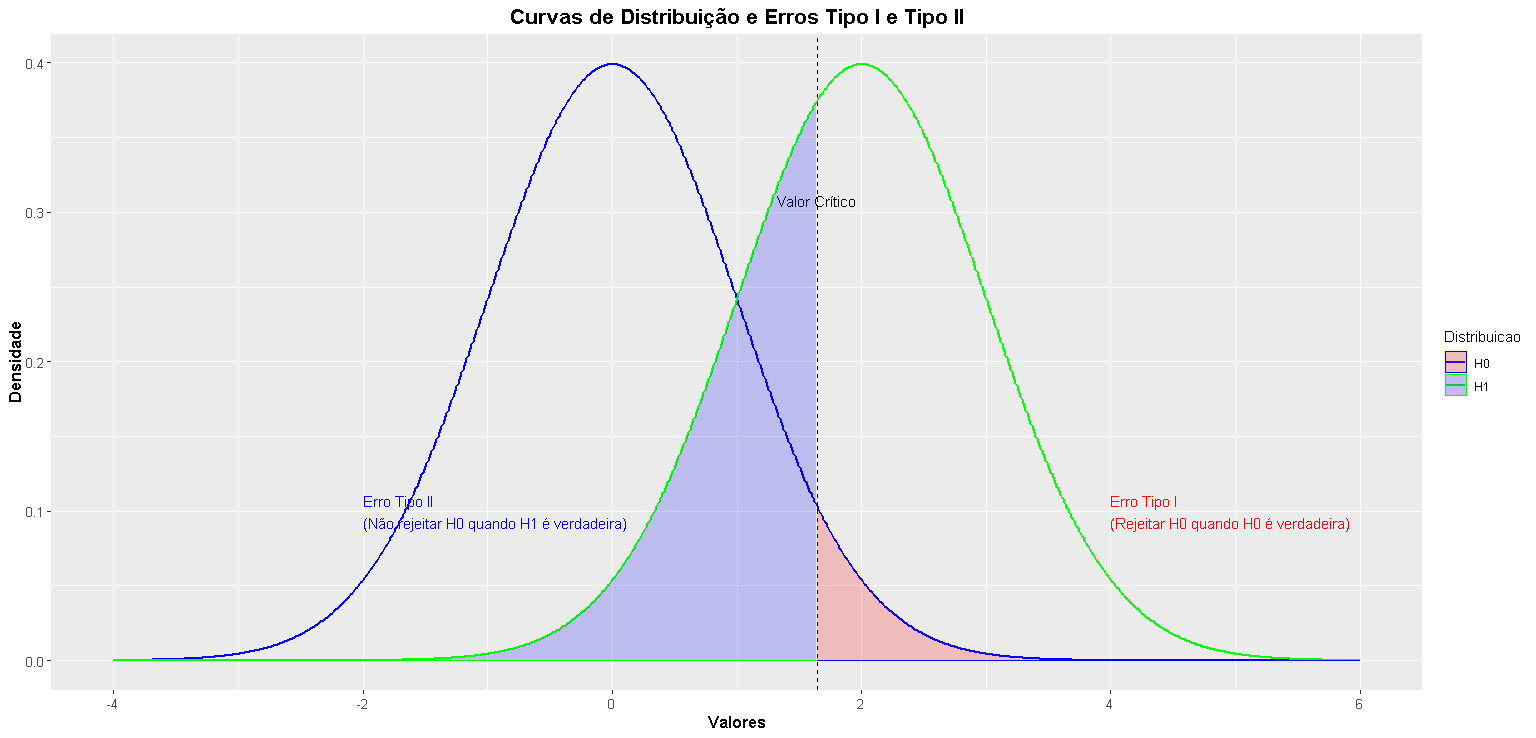
\includegraphics[width=1\linewidth]{../../vis_rep_data/apostila/figs/hyp_test}
	\caption{duas curvas de distribuição de probabilidades, uma para a hipótese nula ($H_0$) e outra para a hipótese alternativa ($H_1$). As áreas sombreadas em vermelho e azul ilustram os erros do Tipo I e do Tipo II, respectivamente.}
	\label{fig:hyptest}
\end{figure}


O equilíbrio entre esses erros é crucial. O nível de significância, muitas vezes fixado em 0,05, ajuda a controlar a taxa de erros do Tipo I. No entanto, a redução dos erros do Tipo I pode aumentar a probabilidade de erros do Tipo II. Assim, a análise estatística não consiste apenas na aplicação de uma fórmula; requer uma consideração cuidadosa do contexto, dos dados e das implicações potenciais de ambos os tipos de erros.

A programação R, com seu conjunto abrangente de ferramentas estatísticas, simplifica a aplicação de testes de hipóteses. Ele não apenas realiza os cálculos necessários, mas também auxilia na visualização dos dados, o que pode fornecer \textit{insights} adicionais. Através do R, podemos executar com eficiência vários testes de hipóteses, desde testes t simples até análises mais complexas, tornando-o uma ferramenta inestimável tanto para estatísticos quanto para analistas de dados.

Em resumo, o teste de hipóteses é um método, que se observado com rigor e correção, suporta a decisão dentro de fatores repetíveis. Requer uma compreensão de conceitos estatísticos como hipóteses nulas e alternativas, valores $p$ e os tipos de erros que podem ocorrer. 

\subsection{Teste de Hipóteses -- Um Exemplo Prático}

Nesta seção, demonstraremos como conduzir um teste de hipóteses\footnote{O teste  apresentado nesta Seção foi extraído de \cite{numberaroundus}.} no R usando um conjunto de dados do mundo real. Exploraremos o conjunto de dados 'PlantGrowth', incluído no R, que contém dados sobre o peso das plantas sob diferentes condições de crescimento. Nosso objetivo será determinar se há uma diferença estatisticamente significativa no crescimento das plantas entre dois grupos de tratamento.





Chapter 2 • An Introduction to Data Analysis
Chapter 3 • Describing Data
Chapter 4 • Central Tendency and Dispersion
Chapter 5 • Univariate and Bivariate Descriptions of Data
Chapter 6 • Transforming Data
Chapter 7 • Some Principles of Displaying Data
Chapter 8 • The Essentials of Probability Theory
Chapter 9 • Confidence Intervals and Testing Hypotheses
Chapter 10 • Making Comparisons
Chapter 11 • Controlled Comparisons

\newpage, 
%\pagebreak
\thispagestyle{plain}
\printpagenotes
\bibliographystyle{unsrt}
\bibliography{vis_rep_data.bib}
\thispagestyle{plain}
\end{document}